\documentclass{crebsshr}

%%%%%%%%% Journal Info -- DO NOT CHANGE %%%%%%%%%
\setcounter{page}{1}
\setcounter{secnumdepth}{4}
\renewcommand\thisnumber{x}
\renewcommand\thisyear{2024}
\renewcommand\thisvolume{x}
\renewcommand\datereceived{}
\renewcommand\dateaccepted{}
\renewcommand\dateavailable{}
\renewcommand\doinumber{10.62366/crebss.2024.x.001}
\renewcommand\type{}
\renewcommand\JEL{, }
%%%%%%%%% End Journal Info %%%%%%%%%

\usepackage[authoryear]{natbib}    % Author-year citations
\usepackage{hyperref}              % Clickable references
\usepackage{graphicx}              % For figures
\usepackage{color}                 % Text color
\usepackage{fontawesome}           % Email icon, if needed
\usepackage{verbatim}              % For verbatim blocks, if needed
\usepackage{booktabs}              % For nicer tables

\begin{document}

\markboth{Sikic}{Dohodovna konvergencija Hrvatske unutar Europske unije: empirijska analiza frakcijske integracije}

\title{Dohodovna konvergencija Hrvatske unutar Europske unije: empirijska analiza frakcijske integracije}

\author[L. Sikic]{Luka Sikic\thanks{Email: \href{mailto:luka.sikic@unicath.hr}{luka.sikic@unicath.hr}}}
\address{\affilnum{1} Croatian Catholic University, Ilica 242, Zagreb, 10000, Croatia}

\keywords{income convergence, convergence clubs, European integration process, fractional integration}

\begin{abstract}
 Rad analizira dohodovnu konvergenciju Hrvatske u razdoblju od 2000.\ do 2024.\ godine prema četiri skupine zemalja: EU15, NMS8, NMS12 i SE4. Korištenjem metodologije vremenskih serija i frakcijske integracije, istražuje se pripadnost Hrvatske različitim konvergencijskim klubovima unutar Europske unije. Rezultati pokazuju da Hrvatska konvergira prema dohodovnim razinama EU15 i SE4, s procijenjenim parametrima frakcijske integracije od 0,87 i 0,95. To ukazuje na spor, ali postojan konvergencijski proces. Međutim, konvergencija prema NMS8 i NMS12 nije potvrđena, s parametrima iznad 1, što sugerira trajne dohodovne razlike. Ovi nalazi impliciraju da se Hrvatska ekonomski približava starim članicama EU i zemljama južne Europe, ali ne i novim zemljama članicama. 
\end{abstract}

\maketitle
\bigskip

%----------------------------------------------------------------------------------
% The main body of the paper
%----------------------------------------------------------------------------------

\section{Uvod}Dohodovna konvergencija predstavlja ključni aspekt ekonomske integracije i razvoja, posebno unutar Europske unije koja teži smanjenju ekonomskih dispariteta među svojim članicama. Za Hrvatsku, kao najnoviju članicu EU, razumijevanje dinamike dohodovne konvergencije je od posebne važnosti. Ovaj rad analizira pripadnost Hrvatske različitim konvergencijskim klubovima unutar EU kako bi se utvrdilo u kojoj mjeri Hrvatska smanjuje dohodovni jaz prema EU. U radu se stoga istražuje  dohodovna konvergencija Hrvatske prema različitim skupinama europskih zemalja: stare članice EU (EU15), nove članice iz srednje i istočne Europe (NMS8 i NMS12) te zemlje južne Europe (SE4). Korištenjem metoda vremenskih serija i frakcijske integracije, istraživanje pruža uvid u konvergencijske procese koji oblikuju ekonomski položaj Hrvatske unutar EU.

Rad doprinosi literaturi na području ekonomske konvergencije kroz nekoliko aspekata. Postojeća literatura o dohodovnoj konvergenciji \citep{aggarwal:23} otkriva nekoliko ključnih praznina koje otežavaju sveobuhvatno razumijevanje regionalnih ekonomskih dinamika, osobito u kontekstu pojedinih zemalja koje prolaze kroz integraciju unutar većih ekonomskih blokova. Jedan značajan nedostatak je ograničeno istraživanje obrazaca konvergencije specifičnih za zemlje koje se prilagođavaju različitim skupinama \citep{cunado:03}, poput Europske unije \citep{brueggemann-trenkler:07}. Većina studija uglavnom se usredotočuje na analize širokog uzorka zemalja, ne ulazeći u detaljne obrasce konvergencije u odnosu na različite podskupine zemalja. Dodatno, metodološka ograničenja ostaju prisutna, kao što je nedostatna primjena ekonometrijskih tehnika koje mogu obuhvatiti složenost procesa konvergencije tijekom duljih razdoblja \citep{granger:80,granger:81,hosking:81}. Tradicionalni pristupi često zanemaruju postojanu i postupnu prirodu prilagodbi dohotka \citep{caselli:96}, što dovodi do pojednostavljenih zaključaka koji ne uzimaju u obzir strukturne i institucionalne razlike među različitim skupinama zemalja. Primjena metodologije vremenskih serija uz frakcijsku integraciju pruža robusno rješenje za ova metodološka i empirijska ograničenja, što se očituje u analizi dohodovne konvergencije Hrvatske od 2000. do 2024. godine. Tehnike frakcijske integracije \citep{cunado:06, ayala:12} omogućuju otkrivanje dugotrajnih ovisnosti i postojanih učinaka u razinama dohotka, pružajući precizniji prikaz dinamike konvergencije u usporedbi s tradicionalnim modelima. Ovaj pristup također omogućuje i procjenu konvergencije Hrvatske prema specifičnim skupinama EU. Korištenjem frakcijske integracije, studija ne samo da rješava ograničenja prijašnjih metodologija već pruža i korisne uvide u specifične obrasce konvergencije Hrvatske u odnosu na različite gospodarske skupine.  

U nastavku rada pruža se pregled ključnih aspekata literature o dohodovnoj konvergenciji te pregled radova koji su analizirali konvergenciju dohotka u europskim posttranzicijskim zemljama. U trećem dijelu opisuju se koncepti dohodovne konvergencije u okviru analize vremenskih serija te se detaljno prikazuje metodologija frakcijske integracije i korišteni procjenitelji. Četvrti dio prikazuje stilizirane činjenice o konvergencijskom procesu Republike Hrvatske prema dohodovnim razinama skupina EU15, NMS8, NMS12 i SE4, dok su u petom dijelu prikazani rezultati istraživanja. U zaključku se sumiraju glavne spoznaje analize.

\section{Pregled literature o dohodovnoj konvergenciji}
Rana literatura o konvergenciji prvenstveno se usmjeravala na provjeru ekonomske teorije rasta \citep{barro-salaimartin:90, barro:92, mankiw:92} koriste\'ci uglavnom prostornu (eng.\ cross-section) regresijsku analizu. Neki autori primijenili su i razli\v{c}ite procjenitelje za panel-podatke \citep{knight:93, islam:95, caselli:96, lee:98, bond:01}. Općenito, rezultati su potvrdili postojanje apsolutne ili uvjetne konvergencije u globalnim uzorcima zemalja, pri \v{c}emu su procijenjene stope konvergencije iznosile izme\dj{}u 2\% i 4\%. Ipak, nije uspostavljen jedinstven konsenzus o globalnoj dohodovnoj konvergenciji.

U kasnijoj fazi, naglasak se pomaknuo na primjenu razli\v{c}itih metoda testiranja dohodovne konvergencije. \cite{bernard-durlauf:91} prvi su analizirali dohodovnu konvergenciju u okviru metodologije vremenskih serija. U kasnijim radovima \citep{bernard-durlauf:96} je istaknuto da tehnike vremenskih serija imaju po\v{z}eljnija empirijska svojstva u odnosu na prostornu analizu. Oni uvode pojam stohasti\v{c}ke konvergencije, koji se odnosi na testiranje jedini\v{c}nog korijena u razlikama BDP-a po stanovniku izme\dj{}u dviju zemalja.

\cite{bernard-durlauf:96} testirali su stohasti\v{c}ku konvergenciju primjenom testova jedini\v{c}nog korijena na razlikama dohotka 15 zemalja OECD-a u odnosu na grupni prosjek. Nisu prona\dj{}eni uvjerljivi dokazi za dugoro\v{c}nu konvergenciju u svim dr\v{z}avama, no potvrdili su konvergenciju za manju skupinu europskih zemalja. \cite{jones:02} je, koriste\'ci metodologiju jedini\v{c}nog korijena i koncept stohasti\v{c}ke konvergencije, analizirao zapadnoafri\v{c}ke dr\v{z}ave te zaklju\v{c}io da ne postoje zna\v{c}ajni dokazi za konvergenciju u cjelokupnom uzorku. \cite{pesaran:06} je primijenio  ADF i KPSS testove stacionarnosti razlika dohotka izme\dj{}u parova zemalja za uzorke od 56, 99 i 101 dr\v{z}ave tijekom razli\v{c}itih razdoblja od 1950. do 2000. godine. U oko 72\% slu\v{c}ajeva potvrdio je konvergencijsku hipotezu, ukazuju\'ci tako na formiranje klubova konvergencije, ali ne i globalnu konvergenicju svih zemalja.

Istra\v{z}ivanja dohodovne konvergencije temeljena na analizi vremenskih serija kasnije su pro\v{s}irena na panel-podatke, uklju\v{c}uju\'ci testove stacionarnosti i kointegracijske analize. \cite{evans-karras:96a} potvrdili su konvergenciju izme\dj{}u 48 ameri\v{c}kih saveznih dr\v{z}ava i 54 zemlje koriste\'ci test jedini\v{c}nog korijena za panel-podatke. U drugom radu, \cite{evans-karras:96b} istra\v{z}ili su apsolutnu konvergenciju izme\dj{}u saveznih dr\v{z}ava SAD-a, no nisu prona\dj{}eni empirijsku potvrdu za taj oblik konvergencije. \cite{fleissig-strauss:01} primijenili su testove jedini\v{c}nog korijena za analizu dugoro\v{c}ne konvergencije u 15 OECD zemalja i europskih zemalja u razdoblju od 1900. do 1987. te zaklju\v{c}ili da je konvergencija potvr\dj{}ena nakon Drugog svjetskog rata, ali ne i za cjelokupni period. \cite{kim:05} je, koriste\'ci panel-kointegracijski test na uzorku od 13 korejskih regija, tako\dj{}er potvrdio konvergenciju, dok su \cite{carrion:05} pomo\'cu panel-testova jedini\v{c}nog korijena zaklju\v{c}ili da postoji konvergencija izme\dj{}u 13 azijskih zemalja.

Relativno mali broj radova o dohodovnoj konvergenciji primijenio je metodologiju frakcijske integracije. Ti su radovi upozorili na ograni\v{c}enja testova jedini\v{c}nog korijena i kointegracije, uglavnom zbog njihove statisti\v{c}ke osjetljivosti te \v{c}injenice da se kointegracijski parametar obi\v{c}no ograni\v{c}ava samo na vrijednosti 0 ili 1. Budu\'ci da je konvergencija proces dugog trajanja, frakcijska integracija nagla\v{s}ava potrebu za variranjem integracijskog parametra u rasponu od 0 do 1 radi obuhvaćanja procesa duge memorije. \cite{michelacci-zaffaroni:00} predla\v{z}u primjenu standardnih testova stacionarnosti kao po\v{c}etni korak u analizi dohodovnih serija, pokazuju\'ci da je u frakcijskom kontekstu konvergencijska stopa od 2\% odgovaraju\'ca za integracijski parametar izme\dj{}u 0,5 i 1. Time su potvrdili rezultate dobivene prostornom regresijskom analizom te zaklju\v{c}ili da je ovaj pristup kompatibilan s metodama vremenskih serija.

U primjeni frakcijske integracije, \cite{cunado:03} ispitali su konvergenciju Australije, Japana, Kanade i Ujedinjenog Kraljevstva prema dohodovnom prosjeku SAD-a. Rezultati su potvrdili konvergenciju za Australiju i Kanadu, dok su za Ujedinjeno Kraljevstvo dokazi bili manje uvjerljivi, a konvergencija za Japan nije mogla biti potvr\dj{}ena. \cite{ayala:12} primijenili su frakcijsku integraciju na uzorak od 17 zemalja Latinske Amerike u odnosu na SAD za razdoblje od 1950. do 2008. godine i nisu prona\dj{}eni dokaze stohasti\v{c}ke konvergencije ni za jednu promatranu zemlju. \cite{fleissig-strauss:01} tako\dj{}er su primijenili frakcijsku integraciju i nisu potvrdili dohodovnu konvergenciju me\dj{}u \v{s}panjolskim regijama.

\subsection{Dohodovna konvergencija u EU posttranzicijskim zemljama}
Istra\v{z}ivanja o dohodovnoj konvergenciji u europskim posttranzicijskim zemljama obuhvatila su raznolike skupine zemalja, razli\v{c}ite aspekte ekonomske konvergencije te su koristila \v{s}irok spektar metodolo\v{s}kih pristupa. Jedna skupina istra\v{z}ivanja fokusirala se na beta i sigma konvergenciju u novim zemljama \v{c}lanicama EU, primjenjuju\'ci prostorne i panel analize, dok su drugi radovi koristili metodologiju vremenskih serija. Razli\v{c}ite duljine analiziranih vremenskih razdoblja me\dj{}u istra\v{z}ivanjima ote\v{z}avale su usporedivost rezultata. Druga skupina istra\v{z}ivanja prou\v{c}avala je konvergenciju raznih makroekonomskih indikatora u posttranzicijskim zemljama prema europskim standardima.

\cite{kocenda:01} analizirao je konvergenciju makroekonomskih indikatora za zemlje Srednje i Isto\v{c}ne Europe prema europskom prosjeku u razdoblju od 1991. do 1998. godine. Rezultati su pokazali konvergenciju u ve\'cini zemalja i indikatora, s najizra\v{z}enijom konvergencijom u dohotku te br\v{z}im napretkom balti\v{c}kih zemalja.  \cite{dobrinsky:01} fokusirao se na dohodovnu konvergenciju novih \v{c}lanica EU, ukazuju\'ci da se pozitivan trend konvergencije prema europskim razinama pojavio nakon sredine 1990-ih godina. \cite{kutan-yigit:03} istra\v{z}ivali su nominalnu i realnu konvergenciju u pet skupina europskih tranzicijskih zemalja u razdoblju od 1993. do 2000. godine, potvr\dj{}uju\'ci ni\v{z}i stupanj nominalne i realne konvergencije. \cite{vojinovic-oplotnik:08} analizirali su uvjetnu beta i sigma konvergenciju zemalja koje su pristupile EU 2004. godine, otkrivaju\'ci ubrzanu konvergenciju u razdoblju od 1995. do 2006. godine. \cite{kocenda:06} ispitali su nominalnu i realnu konvergenciju deset novih \v{c}lanica EU, pri \v{c}emu su utvrdili sporu dohodovnu konvergenciju, ali br\v{z}u nominalnu konvergenciju.

\cite{brueggemann-trenkler:07} primijenili su testove jedini\v{c}nog korijena za analizu dohodovne konvergencije \v{C}e\v{s}ke, Poljske i Ma\dj{}arske prema EU15 i mediteranskim zemljama, potvr\dj{}uju\'ci konvergenciju za \v{C}e\v{s}ku i Ma\dj{}arsku. \cite{rapacki-prochniak:09} istra\v{z}ivali su apsolutnu i uvjetnu beta konvergenciju te sigma konvergenciju u 27 biv\v{s}ih socijalisti\v{c}kih zemalja od 1990. do 2005. godine, zaklju\v{c}uju\'ci da Srednja i Isto\v{c}na Europa imaju razli\v{c}ite konvergencijske obrasce u usporedbi sa zemljama Zajednice nezavisnih dr\v{z}ava (CIS). \cite{ingianni-zdarek:09} analizirali su dohodovnu konvergenciju novih \v{c}lanica EU koriste\'ci razli\v{c}ite metodologije, te su zaklju\v{c}ili da konvergencija postoji, ali nije postojana.  \cite{vojinovic:09} potvrdili su beta i sigma konvergenciju za deset zemalja koje su postale \v{c}lanice EU 2004. godine, s ubrzanom konvergencijom od sredine 1990-ih do 2000-ih, potaknutoj integracijom s EU.

Nekoliko istra\v{z}ivanja potvrdilo je dohodovnu konvergenciju posttranzicijskih zemalja prema europskom centru \citep{monfort:13, rapacki-prochniak:19, szeles-marinescu:10} u razdoblju do posljednjeg pro\v{s}irenja Europske unije. Rezultati istraživanja također ukazuju na nastavak konvergencijskog procesa i nakon globalne financijske krize. Međutim, literatura općenito nije postigla konsenzus o tome hoće li proces konvergencije posttranzicijskih zemalja biti dovršen. Unatoč tome, rezultati sugeriraju da je članstvo u Europskoj uniji bilo ključno za nastavak približavanja tih zemalja europskom dohotovnom prosjeku.

\section{Metodologija}

\subsection{Koncepti dohodovne konvergencije u okviru metodologije vremenskih serija i frakcijska integracija}

U metodologiji vremenskih serija poznata su dva temeljna konvergencijska koncepta: apsolutna i uvjetna konvergencija. Dohodovna konvergencija može se definirati kao:

\begin{equation} \label{eq:eq1}
\lim_{k \to \infty} E(y_{i,t+k} - y_{j,t+k} \mid I_t) = 0
\end{equation}

gdje je dohodak u danom periodu definiran kao \( y_t = \ln(Y_t) \), \( y_{i,t} \) označava dohodak u zemlji \( i \) u trenutku \( t \), \( y_{j,t} \) je dohodak u zemlji \( j \) u istom razdoblju, dok \( I_t \) označava set raspoloživih informacija u danom periodu. Jednadžba (\ref{eq:eq1}) označava da je razlika dohotka zemlje \( i \) i \( j \) stacionaran proces sa prosjekom nula. Ovaj koncept, poznat kao deterministička konvergencija, definirali su  \cite{bernard-durlauf:91}.

Proširenjem definicije (\ref{eq:eq1}):

\begin{equation} \label{eq:eq2}
\lim_{k \to \infty} E(y_{i,t+k} - y_{j,t+k} \mid I_t) = \beta
\end{equation}

gdje \( \beta \) označava konstantu, (\ref{eq:eq1}) predstavlja definiciju apsolutne konvergencije, dok se (\ref{eq:eq2}) odnosi na uvjetnu konvergenciju. Jednadžba (\ref{eq:eq2}) označava da će dvije zemlje konvergirati uz postojanje konstantnog dohodovnog jaza jednakog \( \beta \). Ovaj koncept stohastičke konvergencije, koji su definirali  \cite{carlino-mills:93}, implicira da je razlika dohotka zemalja \( i \) i \( j \) trend stacionaran proces.

Pošto se konvergencijski koncepti (\ref{eq:eq1}) i (\ref{eq:eq2}) odnose na logaritmirane vrijednosti, izražene kao:

\begin{equation} \label{eq:eq3}
\log\left(\frac{y_{i,t}}{y_{j,t}}\right)
\end{equation}

Apsolutna konvergencija prema definiciji (\ref{eq:eq3}) izražava se kao:

\begin{equation} \label{eq:eq4}
\log\left(\frac{y_{i,t}}{y_{j,t}}\right) = \alpha + \epsilon_{i,j,t}
\end{equation}

Uvjetna konvergencija definirana je kao:

\begin{equation} \label{eq:eq5}
\log\left(\frac{y_{i,t}}{y_{j,t}}\right) = \beta + \alpha + \epsilon_{i,j,t}
\end{equation}

Statistička analiza dohodovne konvergencije može se provesti testom jediničnog korijena u vremenskoj seriji razlike dohotka zemalja \( i \) i \( j \), kako predlažu \cite{carlino-mills:93}. Druga metoda je kointegracijska analiza, koju su predložili \cite{bernard-durlauf:91}. Da bi se ekonomski koncepti dohodovne konvergencije ekonometrijski testirali, definiramo:

\begin{equation} \label{eq:eq6}
y_{i,j,t} = \log\left(\frac{Y_{i,t}}{Y_{j,t}}\right)
\end{equation}

gdje \( y_{i,j,t} \) predstavlja razliku logaritama dohotka u zemlji \( i \) i \( j \). Uz definicije dohodovne konvergencije (\ref{eq:eq1}) i (\ref{eq:eq2}) te uzimajući u obzir da \( I_t \) označava informacijski set u trenutku \( t \), jednadžba (\ref{eq:eq6}) se može kompaktno zapisati:

\begin{equation} \label{eq:eq7}
y_{i,j,t} = \alpha + \epsilon_{i,j,t}
\end{equation}

Model (\ref{eq:eq6}) može se asimptotski izraziti kao:

\begin{equation} \label{eq:eq8}
y_{i,j,t} = \beta + \alpha + \epsilon_{i,j,t}
\end{equation}

iz čega slijedi da svaka situacija gdje \( \beta = 0 \) implicira konvergenciju uz konstantnu dohodovnu razliku. Ovo postaje jasnije preuređenjem jednadžbe (\ref{eq:eq8}):

\begin{equation} \label{eq:eq9}
\Delta y_{i,j,t} = \epsilon_{i,j,t}
\end{equation}

\subsection{Frakcijska integracija}

Koncept frakcijske integracije \citep{granger:80,granger:81,granger-joyeux:80,hosking:81} uveden je u makroekonomsku literaturu kako bi se modelirali i autokorelirani procesi za koje je karakteristična povezanost među međusobno udaljenim realizacijama. Ukoliko je neka vremenska serija integrirana reda \( z=0 \), može se reći kako je riječ o procesu kratke memorije čija autokorelacijska funkcija brzo opada, dok integracijski parametar \( z=1 \) označava nestacionarnost i perzistentnost šokova u takvoj vremenskoj seriji. 

Od statističkog i ekonomskog interesa je analizirati da li integracijski parametar poprima neku necjelobrojnu vrijednost unutar intervala \( 0<z<1 \). Primjerice, ukoliko \( 0<z<0.5 \), vremenska serija je stacionarna, no njena autokorelacijska funkcija će opadati sporije nego u slučaju \( z=0 \). Slučaj kada parametar integracije leži u intervalu \( 0.5<z<1 \) označava vremensku seriju koja je nestacionarna, no reverzibilna prema prosjeku. Tada je riječ o procesu duge memorije koji nije kovarijančno stacionaran, no šokovi će ipak nestati iz serije u dugom roku.

\subsection{Frakcijski integrirani proces}

Frakcijski integrirani proces dohodovnih razlika između zemlje \( i \) i \( j \) se može zapisati u obliku:

\begin{equation} \label{eq:eq10}
(1-L)^z (y_{i,t} - y_{j,t}) = \epsilon_t
\end{equation}

gdje je \( L \) operator pomaka i definiran je kao \( L^k y_t = y_{t-k} \), \( \epsilon_t \) označava standardnu pogrešku modela za koju se pretpostavlja da je opisana stohastičkim procesom bijelog šuma koji ima prosjek nula i konstantnu varijancu.

Jednadžbu (\ref{eq:eq10}) je sada moguće izraziti u generalnijem obliku pogodnom za empirijsko testiranje:

\begin{equation} \label{eq:eq11}
\phi(L)(1-L)^z (y_{i,t} - y_{j,t}) = \theta(L)\epsilon_t
\end{equation}

gdje je \( \phi(L) \) autoregresivni polinom pomaka definiran kao \( \phi(L) = 1 - \phi_1 L - \phi_2 L^2 - \dots - \phi_p L^p \), \( \theta(L) \) je polinom pomičnog prosjeka operatora pomaka i opisan je kao \( \theta(L) = 1 + \theta_1 L + \theta_2 L^2 + \dots + \theta_q L^q \), dok \( (1-L)^z \) predstavlja operator frakcijske diferencije u obliku:

\begin{equation} \label{eq:eq12}
(1-L)^z = \sum_{k=0}^{\infty} \frac{\Gamma(k-z)}{\Gamma(-z)\Gamma(k+1)} L^k
\end{equation}

Pri tome \( \Gamma(\cdot) \) označava generaliziranu faktorsku gama funkciju.

Invertiranje jednadžbe (\ref{eq:eq11}) je moguće u slučaju kada parametar \( z \) frakcijske integracije leži u intervalu \( 0<z<0.5 \), te je tada moguće je zapisati:

\begin{equation} \label{eq:eq13}
y_{i,t} - y_{j,t} = \frac{\theta(L)}{\phi(L)}(1-L)^{-z}\epsilon_t
\end{equation}

iz čega je vidljivo da \( \phi(L) \) opisuje kratkoročnu dinamiku procesa, dok su njegovi dugoročni efekti obuhvaćeni izrazom za frakcijsku integraciju \( (1-L)^{-z} \).

U slučaju kada je \( z \) invertibilnost u (\ref{eq:eq13}) moguća, proces (\ref{eq:eq11}) je stacionaran. U kontekstu ovog rada je od posebnog interesa slučaj u kojem parametar frakcijske integracije leži u intervalu \( 0.5<z<1 \). Tada je riječ o nestacionarnom procesu koji ima tendenciju vraćanja prema prosjeku (mean-reverting).

Za proces koji ima tendenciju vraćanja prema prosječnoj vrijednosti je karakteristično da funkcija kumulativnih impulsnih šokova asimptotski teži nuli. Upravo se tu očituje dodatna fleksibilnost pristupa frakcijske kointegracije u odnosu na pristup testiranja stacionarnosti ili kointegracije.

Naime, parametar frakcijske integracije koji iznosi manje od jediničnog označava kako će šok vremenske serije \( \epsilon_t \) odumrijeti čak i u slučaju da je ta vremenska serija ima karakteristike nestacionaranog procesa. \cite{mello-guimaraes:07} dokazuju kako je u tom slučaju koncept uvjetne dohodovne konvergencije dobro opisan frakcijski integriranim procesom (\ref{eq:eq11}).

\subsection{Empirijska specifikacija}

Empirijska specifikacija konvergencije se u ovom radu odnosi na dohodovni diferencijal između Hrvatske i dohodovnog prosjeka četiri grupe zemalja EU15, NMS8, NMS12 te SE4. Budući da se prosjek grupe zemalja koristi kao konvergencijski benchmark, model (\ref{eq:eq6}) je potrebno preinačiti na način:

\begin{equation} \label{eq:eq14}
\phi(L)(1-L)^z (\log y_{HR,t} - \log y_{avg,t}) = \theta(L)\epsilon_t
\end{equation}

gdje \( \log y_{avg,t} \) označava dohodovni prosjek \( j \) zemalja svake od četiri navedene grupe i definiran je kao:

\begin{equation} \label{eq:eq15}
\log y_{avg,t} = \frac{1}{n}\sum_{j=1}^{n} \log y_{j,t}
\end{equation}

To implicira konačnu empirijsku specifikaciju dohodovnog diferencijala u obliku:

\begin{equation} \label{eq:eq16}
y_{HR,t} - y_{avg,t} = \frac{\theta(L)}{\phi(L)}(1-L)^{-z}\epsilon_t
\end{equation}


\section{Korišteni podaci i stilizirane činjenice o konvergencijskom procesu Hrvatske}

U istraživanju se koriste vremenske serije BDP-a Hrvatske i nekoliko skupina zemalja u razdoblju od početka 2000.\ do kraja 2023.\ godine: stare zemlje članice Europske Unije (EU15), nove zemlje članice (NMS8 i NMS12) te zemlje juga Europe (SE4). Pri tome se koriste EUROSTAT-ovi podatci BDP-a na kvartalnoj frekvenciji u razdoblju od 2000q1 do 2023q4. EUROSTAT baza objavljuje podatke za kvartalni BDP bez korekcije za broj stanovnika pa je zbog toga dodatno korištena IMF-ova baza World Economic Outlook iz koje su preuzeti godišnji podatci o stanovništvu u periodu od 2000.\ godine do 2023.\ godine za sve zemlje obuhvaćene analizom. Godišnji podatci za stanovništvo su metodom kubične interpolacije svedeni na kvartalne, nakon čega su korišteni u formiranju vremenske serije BDP per capita na kvartalnoj frekvenciji.

\begin{figure}[ht]
\centering
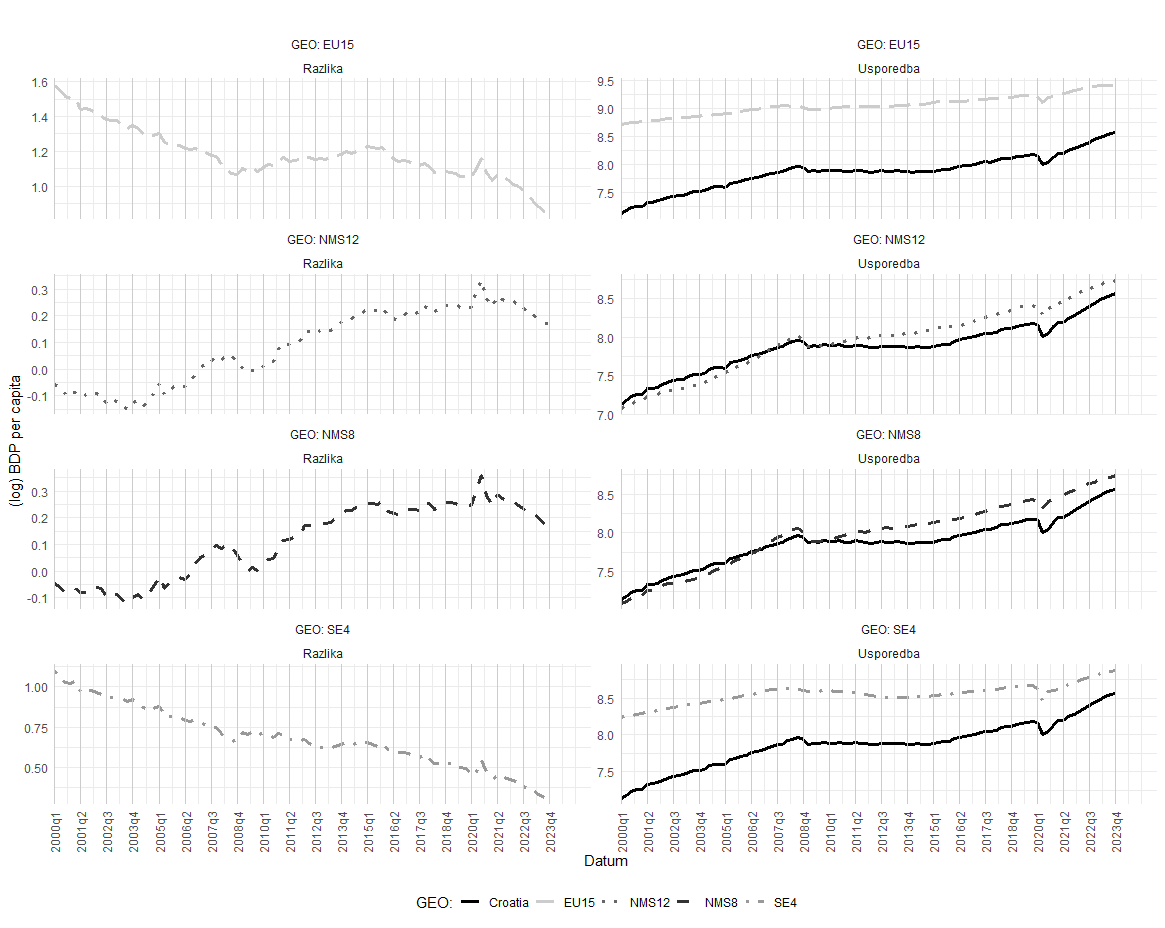
\includegraphics[width=\linewidth]{Rplot.png} % Zamijenite 'Rplot.png' sa stvarnom putanjom vaše slike
\caption{Kretanje razlika u BDP-u po stanovniku između Hrvatske i analiziranih skupina zemalja.}
\label{fig:grafikon1}
\end{figure}

Slika \ref{fig:grafikon1} pruža vizualni prikaz kretanja razlika u BDP-u po stanovniku između Hrvatske i analiziranih skupina zemalja. U gornjem panelu prikazano je kretanje BDP-a po stanovniku za Hrvatsku i EU15. Do globalne ekonomske krize 2007.\ godine, Hrvatska je bilježila brži rast BDP-a, značajno se približavajući prosjeku EU15. Međutim, nakon izbijanja krize dolazi do korekcije hrvatskog BDP-a. Dok se EU15 postupno oporavlja i nastavlja s rastom, hrvatski dohodak stagnira ili čak opada. U novijem razdoblju, nakon krize uzrokovane pandemijom COVID-19, hrvatski BDP ponovno ubrzava rast, pokazujući obnovljeni trend približavanja prosjeku EU15.

Središnja dva panela prikazuju usporedbu Hrvatske s NMS8 i NMS12. Zanimljivo je da su do 2007.\ godine sve zemlje imale podjednake stope rasta, sugerirajući zajedničku konvergenciju. No, nakon krize, hrvatsko gospodarstvo počinje usporavati ili stagnirati, dok NMS8 i NMS12 bilježe nastavak snažnijeg rasta. To je rezultiralo rastućim jazom između BDP Hrvatske i tih dviju skupina. Ipak, u novije vrijeme, osobito nakon COVID-19 krize, primjetan je novi zamah u hrvatskom gospodarstvu, što dovodi do ublažavanja dohodovnog jaza u odnosu na NMS8 i NMS12. Zadnji panel pruža pregled odnosa Hrvatske prema SE4 skupini. Tijekom cijelog promatranog razdoblja vidljiva je stabilnija konvergencija: unatoč kratkotrajnom usporavanju tijekom krize 2007.\ godine, Hrvatska je kontinuirano bilježila brži rast od SE4, potvrđujući dugoročnu tendenciju konvergiranja prema toj skupini.

Iz prikazanih podataka može se zaključiti kako Hrvatska u dugom roku nastavlja konvergirati prema prosjeku EU15 i SE4. Iako je konvergencija prema NMS8 i NMS12 neko vrijeme bila zaustavljena ili usporena, osobito od 2007.\ do razdoblja nakon COVID-19 krize, najnoviji podatci upućuju na to da je i prema tim skupinama ponovno započeo proces približavanja. Kriza iz 2007.\ godine zaustavila je konvergenciju prema EU15 samo privremeno, dok je kretanje prema SE4 ostalo postojano. U novijem, postpandemijskom razdoblju, Hrvatska pokazuje pojačanu gospodarsku vitalnost, podržavajući daljnje smanjenje dohodovnih razlika u odnosu na sve analizirane skupine zemalja.

%==========================================================================================================================================
\section{Rezultati analize}

Nakon deskriptivne analize podataka, u ovom dijelu predstavljeni su rezultati statističkih testova dohodovne konvergencije između Hrvatske i skupina EU15, NMS8, NMS12 te SE4. Rezultati su dobiveni korištenjem proširenog Dickey-Fuller (ADF) testa te procjenitelja frakcijske integracije koji su predložili \cite{geweke-porter:83}. Prije provođenja ovih statističkih testova, provedeni su Ljung-Box test i analiza autokorelacijske funkcije (ACF) za 20 vremenskih zaostataka kako bi se procijenila prikladnost korištene metodologije.

\begin{table}[ht]
\centering
\caption{Ljung-Box Test, P-val}
\label{tab:tablica1}
\begin{tabular}{lcccccccccc}
\toprule
\textbf{Group} & \textbf{Lag 2} & \textbf{Lag 4} & \textbf{Lag 6} & \textbf{Lag 8} & \textbf{Lag 10} & \textbf{Lag 12} & \textbf{Lag 14} & \textbf{Lag 16} & \textbf{Lag 18} & \textbf{Lag 20} \\
\midrule
EU15  & 0 & 0 & 0 & 0 & 0 & 0 & 0 & 0 & 0 & 0 \\
NMS12 & 0 & 0 & 0 & 0 & 0 & 0 & 0 & 0 & 0 & 0 \\
NMS8  & 0 & 0 & 0 & 0 & 0 & 0 & 0 & 0 & 0 & 0 \\
SE4   & 0 & 0 & 0 & 0 & 0 & 0 & 0 & 0 & 0 & 0 \\
\bottomrule
\end{tabular}
\end{table}

Tablica \ref{tab:tablica1} prikazuje p-vrijednosti od 0 za sve vremenske zaostatke u Ljung-Box testu, što ukazuje na odbacivanje nulte hipoteze o nepostojanju autokorelacije. Ovaj rezultat sugerira značajnu autokorelaciju kroz sve vremenske zaostatke, implicirajući da prošle vrijednosti imaju snažan i statistički značajan utjecaj na buduće vrijednosti tijekom cijelog promatranog razdoblja. Prisustvo autokorelacije na višestrukim zaostacima ukazuje da podatke karakterizira dugo pamćenje ili perzistentnost, što znači da se utjecaj prošlih šokova sporo smanjuje tijekom vremena, a povijesne vrijednosti serije nastavljaju utjecati na buduća opažanja kroz dulje vremensko razdoblje.

S obzirom na ovako izraženu strukturu autokorelacije, konvencionalni modeli vremenskih serija koji pretpostavljaju procese kratkog pamćenja neće adekvatno uvažiti temeljnu dinamiku podataka. Stoga je nužno primijeniti modele koji mogu uzeti u obzir dugoročne ovisnosti, poput procjenitelja frakcijske integracije, koji su prikladni za modeliranje i predviđanje u prisutnosti karakteristika dugog pamćenja.

\begin{figure}[ht]
\centering
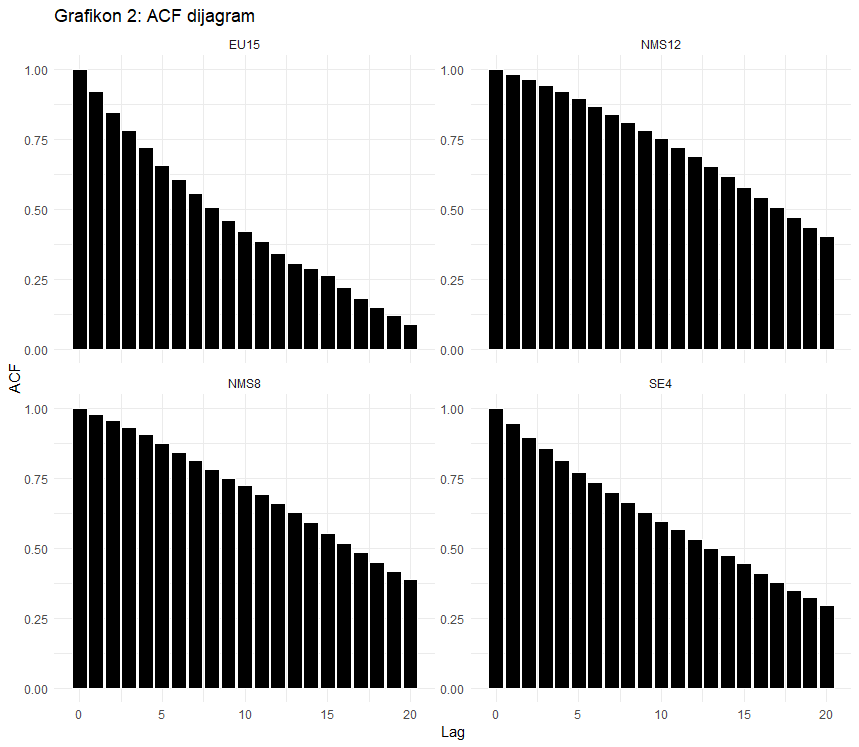
\includegraphics[width=\linewidth]{Rplot01.png} % Zamijenite 'Rplot01.png' sa stvarnom putanjom vaše slike
\caption{Autokorelacijske funkcije (ACF) za sve četiri analizirane skupine.}
\label{fig:grafikon2}
\end{figure}

Slika \ref{fig:grafikon2} prikazuje autokorelacijske funkcije (ACF) vremenskih serija za sve četiri analizirane skupine (EU15, NMS8, NMS12, SE4). Uočava se konzistentan obrazac u svim serijama: visoka autokorelacija pri nižim zaostacima koja se postupno smanjuje s povećanjem broja zaostataka. Ovaj obrazac potvrđuje da svaku vremensku seriju karakterizira značajna autokorelacija koja se proteže preko više vremenskih zaostataka. Štoviše, sporo opadanje vrijednosti ACF dodatno potkrepljuje prisutnost dugog pamćenja i perzistentnosti u podacima.

Ovi nalazi naglašavaju važnost uvažavanja dugoročnih ovisnosti u analizi dohodovne konvergencije. Perzistentnost koju sugeriraju ACF grafikoni ukazuje na to da šokovi u dohodovnim diferencijalima između Hrvatske i odgovarajućih skupina zemalja imaju trajne učinke, te se frakcijska integracija nameće kao prikladna metoda za uvažavanje ovakve konvergencijske dinamike.

\begin{table}[ht]
\centering
\caption{ADF Test}
\label{tab:tablica2}
\begin{tabular}{lccc}
\toprule
\textbf{Group Name} & \textbf{Bez kons/tr} & \textbf{Konst} & \textbf{Konst/tr} \\
\midrule
RH-NMS8  & -0.3342 & -1.2816 & -1.2669 \\
RH-NMS12 & -0.2698 & -1.0464 & -1.3638 \\
RH-SE4   & -4.1785*** & -0.7209 & -2.6062* \\
RH-EU15  & -2.97** & -1.2619 & -1.9528 \\
\bottomrule
\end{tabular}
\\
\footnotesize{*** p < 0.01, ** p < 0.05, * p < 0.1}
\end{table}

Tablica \ref{tab:tablica2} prikazuje rezultate ADF testa jediničnog korijena primijenjenog na vremenske serije dohodovnih diferencijala između Hrvatske i četiri grupe zemalja. Kroz specificiranje različitih determinističkih komponenti u testnim jednadžbama, omogućeno je testiranje različitih oblika dohodovne konvergencije: apsolutne konvergencije, uvjetne konvergencije te konvergencije prema determinističkom trendu.

Apsolutna konvergencija testira se specifikacijom bez konstante i trenda, gdje ADF test ispituje stacionarnost oko nulte razlike u BDP-u. Rezultati pokazuju da su testne statistike za parove RH-NMS8 (-0,3342) i RH-NMS12 (-0,2698) nedovoljno značajne, što ne omogućuje odbacivanje nulte hipoteze o postojanju jediničnog korijena. Ovi nalazi sugeriraju odsutnost dokaza o apsolutnoj konvergenciji između Hrvatske i grupa NMS8 te NMS12. Nasuprot tome, testne statistike za parove RH-SE4 (-4,1785\textsuperscript{***}) i RH-EU15 (-2,97\textsuperscript{**}) su značajne na razinama od 1\% i 5\%, što ukazuje na postojanje apsolutne konvergencije između Hrvatske i grupa SE4 te EU15.

Uvjetna konvergencija ispituje se uključivanjem konstante u specifikaciju, gdje ADF test procjenjuje stacionarnost oko nenulte razlike u BDP-u. Rezultati pokazuju da niti jedna testna statistika za parove RH-NMS8 (-1,2816), RH-NMS12 (-1,0464), RH-SE4 (-0,7209) i RH-EU15 (-1,2619) nije značajna na uobičajenim razinama. Ovo upućuje na nedostatak dokaza o uvjetnoj konvergenciji između Hrvatske i analiziranih skupina zemalja.

Konvergencija prema determinističkom trendu ispituje se specifikacijom koja uključuje i konstantu i trend, gdje ADF test procjenjuje stacionarnost oko determinističkog trenda, što implicira konvergenciju prema zajedničkoj putanji rasta. Rezultati pokazuju da testne statistike za parove RH-NMS8 (-1,2669) i RH-NMS12 (-1,3638) nisu statistički značajne, što sugerira odsutnost konvergencije Hrvatske s ovim zemljama prema zajedničkom trendu. Za par RH-SE4, testna statistika iznosi -2,6062\textsuperscript{*}, što je značajno na razini od 10\%, dok je za par RH-EU15 testna statistika -1,9528, što također ne omogućuje odbacivanje nulte hipoteze o jediničnom korijenu.

\begin{table}[ht]
\centering
\caption{Rezultati GPH testa za različite širine pojasa}
\label{tab:tablica4}
\begin{tabular}{lcccccc}
\toprule
\textbf{Naziv grupe} & \textbf{GPH d (0.4)} & \textbf{GPH d (0.5)} & \textbf{GPH d (0.6)} & \textbf{GPH d (0.7)} & \textbf{GPH d (0.8)} & \textbf{GPH d (0.9)} \\
\midrule
Croatia vs NMS8   & 1.4347*** & 1.1921*** & 1.286***  & 1.1137*** & 1.1511*** & 1.1446*** \\
Croatia vs NMS12  & 1.5002*** & 1.2523*** & 1.2915*** & 1.1047*** & 1.1534*** & 1.1048*** \\
Croatia vs SE4    & 0.8852*** & 0.8712*** & 0.8867*** & 0.9279*** & 0.9272*** & 0.9516*** \\
Croatia vs EU15   & 0.5643*** & 0.6541*** & 0.7256*** & 0.8405*** & 0.8554*** & 0.8986*** \\
\bottomrule
\end{tabular}
\\
\footnotesize{*** p < 0.01, ** p < 0.05, * p < 0.1}
\end{table}
Tablica \ref{tab:tablica4} prikazuje rezultate testa dohodovne konvergencije temeljenog na specifikaciji modela frakcijske integracije. Test je primijenjen na različite širine pojasa (od 0,4 do 0,9) kako bi se robusno ispitale serije dohodovnih diferencijala između Hrvatske i četiri grupe zemalja: NMS8, NMS12, SE4 te EU15. Parametar d pruža uvid u memorijske karakteristike, odnosno perzistentnost, analiziranih vremenskih serija, što ima izravne implikacije za razumijevanje dohodovne konvergencije. Parametar d interpretira se na sljedeći način: kada je d < 0,5, serija je stacionarna i pokazuje kratku memoriju, što znači da šokovi imaju privremene učinke. Kada je d u rasponu od 0,5 do 1, serija je nestacionarna, ali se vraća svojoj sredini, implicirajući da šokovi imaju dugotrajne, ali ne trajne učinke. Vrijednost d = 1 označava da serija ima jedinični korijen, što znači da šokovi imaju trajne učinke. Za vrijednosti d > 1, serija je nestacionarna, ne vraća se svojoj sredini te pokazuje eksplozivno ponašanje, što također implicira trajne učinke šokova.

Za grupe NMS8 i NMS12, procijenjene vrijednosti parametra $d$ su konzistentno veće od 1 kroz sve širine pojasa, krećući se u rasponu od 1,1137\textsuperscript{***} do 1,4347\textsuperscript{***} za NMS8 i od 1,1047\textsuperscript{***} do 1,5002\textsuperscript{***} za NMS12, te su statistički značajne na razini od 1\%. To ukazuje da su serije dohodovnih diferencijala između Hrvatske i ovih grupa nestacionarne i ne vraćaju se na srednju vrijednost. Takav rezultat implicira nepostojanje konvergencije, perzistentnost šokova te trajna odstupanja u razinama dohotka. 

Procijenjene vrijednosti $d$ za grupu SE4 kreću se od približno 0,8852\textsuperscript{***} do 0,9516\textsuperscript{***} i sve su značajne na razini od 1\%. Takav rezultat implicira da je serija nestacionarna, ali se vraća srednjoj vrijednosti. To znači da, iako šokovi imaju dugotrajne učinke, dohodovne će se razlike smanjivati tijekom vremena. 

Za grupu EU15, procijenjene vrijednosti parametra $d$ se povećavaju od približno 0,5643\textsuperscript{***} do 0,8986\textsuperscript{***} kako se širina pojasa povećava, i sve su značajne na razini od 1\%. Ovakvi rezultati sugeriraju da se serija dohodovnih diferencijala vraća na srednju vrijednost, što implicira postojanje konvergencije.

Rezultati testa frakcijske integracije potvrđuju zaključak o postojanju uvjetne dohodovne konvergencije između Hrvatske i EU15 te djelomično između Hrvatske i SE4, dok to nije potvrđeno za NMS8 i NMS12. Konvergencijska dinamika između Hrvatske i EU15 je prisutna, ali izuzetno spora, što je naznačeno vrijednostima parametra $d$ bližima 1. Konvergencija sa SE4 je nešto brža, ali rezultati zahtijevaju daljnju analizu zbog blizine vrijednosti parametra $d$ kritičnoj granici. Parametar frakcijske integracije viši od 0,5 označava spor konvergencijski proces, dok vrijednosti bliže jediničnoj sugeriraju usporavanje tog procesa. To implicira da, iako postoji tendencija smanjenja dohodovnih razlika, dinamika konvergencije je takva da će biti potreban dugi vremenski period za postizanje značajnih rezultata.

Implikacije ovih rezultata valja tumačiti u kontekstu europskih integracijskih procesa. Unatoč kasnijem pristupanju Europskoj uniji, Hrvatska je primjenjivala slične mjere institucionalnog, pravnog i ekonomskog usklađivanja kao i nove članice EU iz grupa NMS8 i NMS12. Očekivalo se formiranje konvergencijskog kluba među ovim zemljama, no analiza to nije mogla potvrditi. Ovaj nalaz sugerira da institucionalna i pravna integracija ne rezultiraju nužno i ekonomskom konvergencijom, te da postoje duboko ukorijenjene strukturne razlike koje ometaju taj proces. Potvrda konvergencijske hipoteze za Hrvatsku i EU15 ukazuje da Hrvatska postupno smanjuje dohodovni jaz s razvijenijim članicama EU. Iako je proces spor, prisutnost konvergencijske dinamike postoji. Na kraju, brža konvergencija Hrvatske prema SE4 sugerira da se Hrvatska pridružuje konvergencijskom klubu zemalja južne Europe, koji karakteriziraju niže stope rasta i općenito slični ekonomski izazovi.

\section{Zaključak}
Rad je analizirao dohodovnu konvergenciju Hrvatske s različitim skupinama zemalja Europske unije koristeći analizu vremenskih serija i metode frakcijske integracije. Dok je prethodna literatura pokazala postojanje dohodovne konvergencije za neke, ali ne sve posttranzicijske europske zemlje prema prosjeku EU, ovaj rad proširio je to područje fokusirajući se na konvergencijske obrasce specifične za Hrvatsku. Dodatno, pitanje dohodovne konvergencije smješteno je u širi kontekst europskih integracijskih procesa kroz analizu međusobne konvergencije između Hrvatske i prosjeka dohotka četiri grupe zemalja: EU15, NMS8, NMS12 i SE4. Time je omogućeno zaključivanje o smjeru ekonomske i institucionalne konvergencije unutar europskih integracija te o pripadnosti Hrvatske određenim konvergencijskim klubovima.

Rezultati testova frakcijske integracije dohodovnog diferencijala između Hrvatske i odabranih skupina zemalja pokazali su da konvergencija postoji između Hrvatske i EU15 te Hrvatske i SE4, dok ona nije potvrđena između Hrvatske i NMS8 te NMS12. Svi rezultati su robusni s obzirom na različite procjenitelje i različite izbore širine pojasa. Nalazi impliciraju da je konvergencija Hrvatske prema prosjeku EU15 i SE4 spor proces, ali nešto brži prema SE4. Također se nameće i zaključak da Hrvatska ne pripada konvergencijskom klubu novih članica (NMS8 i NMS12), već konvergencijskim klubovima EU15 i SE4, pri čemu je konvergencija prema SE4 robusnija i brža nego prema EU15.

Ovi nalazi imaju implikacije za europske integracijske procese. Unatoč kasnijem pristupanju Europskoj uniji i primjeni mjera institucionalnog, pravnog i ekonomskog usklađivanja s novim članicama, Hrvatska ne pokazuje dohodovnu konvergenciju s grupama NMS8 i NMS12. To sugerira da institucionalna i pravna integracija ne rezultiraju nužno i ekonomskom konvergencijom. Čini se da Hrvatska ekonomski konvergira prema zemljama EU15 i SE4, koje karakteriziraju sporiji ili negativan gospodarski rast. Potvrda konvergencije prema SE4 ukazuje na pridruživanje Hrvatske konvergencijskom klubu južne Europe i općenito ukazuje na potrebu za politikama koje će potaknuti brži gospodarski rast i razvoj. Ovi nalazi naglašavaju važnost uvažavanja dugoročnih ovisnosti u analizi dohodovne konvergencije. Perzistentnost koju sugeriraju ACF grafikoni ukazuje na to da šokovi u dohodovnim diferencijalima između Hrvatske i odgovarajućih skupina zemalja imaju trajne učinke, te se frakcijska integracija nameće kao prikladna metoda za uvažavanje ovakve konvergencijske dinamike.



\newpage

%--------------------------------------------------------------------------------
% BIBLIOGRAPHY
%--------------------------------------------------------------------------------
\begin{thebibliography}{99}
\small  % If your .cls style sets references in smaller font, keep this

\bibitem[Aggarwal(2023)]{aggarwal:23}
Aggarwal, S. (2023). Convergence of income: A review of the literature.
\emph{European Economic Letters (EEL)}, 13(5):1918--1927.
Dostupno na: \url{https://www.eelet.org.uk/index.php/journal/article/view/1066}

\bibitem[Ayala i sur.(2012)]{ayala:12}
Ayala, A., Cuñado, J. i Gil-Alana, L.A. (2012). Real convergence in Latin America:
a fractionally integrated approach. \emph{Applied Financial Economics}, 22(20):1713--1717.
\href{https://doi.org/10.1080/09603107.2012.674204}{doi: 10.1080/09603107.2012.674204}

\bibitem[Barro i Sala-i-Martin(1990)]{barro-salaimartin:90}
Barro, R. i Sala-i-Martin, X. (1990). Economic Growth and Convergence across The United States.
\href{https://doi.org/10.3386/w3419}{doi: 10.3386/w3419}

\bibitem[Barro(1992)]{barro:92}
Barro, R.J. (1992). Convergence. \emph{Journal of Political Economy}, 100(2):223--251.
\href{https://doi.org/10.1086/261816}{doi: 10.1086/261816}

\bibitem[Begović(2017)]{begovic:17}
Begović, B. (2017). Europe’s Growth Challenge by Anders Åslund and Simeon Djankov.
\emph{Panoeconomicus}, 64(3):371--381.
Dostupno na: \url{https://ideas.repec.org/a/voj/journl/v64y2017i3p371-381.html}

\bibitem[Bernard i Durlauf(1991)]{bernard-durlauf:91}
Bernard, A. i Durlauf, S. (1991). Convergence of international output movements.
\href{https://doi.org/10.3386/w3717}{doi: 10.3386/w3717}

\bibitem[Bernard i Durlauf(1996)]{bernard-durlauf:96}
Bernard, A.B. i Durlauf, S.N. (1996). Interpreting tests of the convergence hypothesis.
\emph{Journal of Econometrics}, 71(1--2):161--173.
\href{https://doi.org/10.1016/0304-4076(94)01699-2}{doi: 10.1016/0304-4076(94)01699-2}

\bibitem[Bond i sur.(2001)]{bond:01}
Bond, S., Hoeffler, A. i Temple, J. (2001). GMM Estimation of Empirical growth Models.
\emph{Economics Papers} [Preprint].
Dostupno na: \url{https://ideas.repec.org/p/nuf/econwp/0121.html}

\bibitem[Brüggemann i Trenkler(2007)]{brueggemann-trenkler:07}
Brüggemann, R. i Trenkler, C. (2007). Are Eastern European countries catching up?
Time series evidence for Czech Republic, Hungary and Poland.
\emph{Applied Economics Letters}, 14(4):245--249.
\href{https://doi.org/10.1080/13504850500425782}{doi: 10.1080/13504850500425782}

\bibitem[Carlino i Mills(1993)]{carlino-mills:93}
Carlino, G.A. i Mills, L.O. (1993). Are U.S. regional incomes converging?
\emph{Journal of Monetary Economics}, 32(2):335--346.
\href{https://doi.org/10.1016/0304-3932(93)90009-5}{doi: 10.1016/0304-3932(93)90009-5}

\bibitem[Carrion-i-Silvestre i sur.(2005)]{carrion:05}
Carrion-i-Silvestre, J.L., Del Barrio-Castro, T. i López-Bazo, E. (2005).
Breaking the panels: An application to the GDP per capita.
\emph{Econometrics Journal}, 8(2):159--175.
\href{https://doi.org/10.1111/j.1368-423x.2005.00158.x}{doi: 10.1111/j.1368-423x.2005.00158.x}

\bibitem[Caselli i sur.(1996)]{caselli:96}
Caselli, F., Esquivel, G. i Lefort, F. (1996). Reopening the convergence debate:
A new look at cross-country growth empirics.
\emph{Journal of Economic Growth}, 1(3):363--389.
\href{https://doi.org/10.1007/bf00141044}{doi: 10.1007/bf00141044}

\bibitem[Cuñado i sur.(2006)]{cunado:06}
Cuñado, J., Gil-Alana, L.A. i De Gracia, F.P. (2006). Additional empirical evidence on real
convergence: a fractionally integrated approach.
\emph{Review of World Economics}, 142(1):67--91.
\href{https://doi.org/10.1007/s10290-006-0057-9}{doi: 10.1007/s10290-006-0057-9}

\bibitem[Cuñado i sur.(2003)]{cunado:03}
Cuñado, J., Gil-Alana, L.A. i De Gracia, F.Pé. (2003). Empirical evidence on real convergence
in some OECD countries.
\emph{Applied Economics Letters}, 10(3):173--176.
\href{https://doi.org/10.1080/1350485022000044066}{doi: 10.1080/1350485022000044066}

\bibitem[Dobrinsky(2001)]{dobrinsky:01}
Dobrinsky, R. (2001). Convergence in Per Capita Income Levels, Productivity Dynamics and
Real Exchange Rates in the Candidate Countries on the Way to EU Accession.
\emph{Empirica} [Preprint]. 
Dostupno na: \url{http://pure.iiasa.ac.at/id/eprint/6484/}

\bibitem[Evans i Karras(1996a)]{evans-karras:96a}
Evans, P. i Karras, G. (1996a). Convergence revisited.
\emph{Journal of Monetary Economics}, 37(2):249--265.
\href{https://doi.org/10.1016/s0304-3932(96)90036-7}{doi: 10.1016/s0304-3932(96)90036-7}

\bibitem[Evans i Karras(1996b)]{evans-karras:96b}
Evans, P. i Karras, G. (1996b). Do economies converge? Evidence from a panel of U.S. states.
\emph{The Review of Economics and Statistics}, 78(3):384.
\href{https://doi.org/10.2307/2109785}{doi: 10.2307/2109785}

\bibitem[Fleissig i Strauss(2001)]{fleissig-strauss:01}
Fleissig, A. i Strauss, J. (2001). Panel Unit-Root Tests of OECD Stochastic Convergence.
\emph{Review of International Economics}, 9(1):153--162.
\href{https://doi.org/10.1111/1467-9396.00270}{doi: 10.1111/1467-9396.00270}

\bibitem[Geweke i Porter-Hudak(1983)]{geweke-porter:83}
Geweke, J. i Porter-Hudak, S. (1983). The estimation and application of long memory
time series models.
\emph{Journal of Time Series Analysis}, 4(4):221--238.
\href{https://doi.org/10.1111/j.1467-9892.1983.tb00371.x}{doi: 10.1111/j.1467-9892.1983.tb00371.x}

\bibitem[Granger(1980)]{granger:80}
Granger, C.W.J. (1980). Long memory relationships and the aggregation of dynamic models.
\emph{Journal of Econometrics}, 14(2):227--238.
\href{https://doi.org/10.1016/0304-4076(80)90092-5}{doi: 10.1016/0304-4076(80)90092-5}

\bibitem[Granger(1981)]{granger:81}
Granger, C.W.J. (1981). Some properties of time series data and their use
in econometric model specification.
\emph{Journal of Econometrics}, 16(1):121--130.
\href{https://doi.org/10.1016/0304-4076(81)90079-8}{doi: 10.1016/0304-4076(81)90079-8}

\bibitem[Granger i Joyeux(1980)]{granger-joyeux:80}
Granger, C.W.J. i Joyeux, R. (1980). An introduction to long-memory time series models
and fractional differencing.
\emph{Journal of Time Series Analysis}, 1(1):15--29.
\href{https://doi.org/10.1111/j.1467-9892.1980.tb00297.x}{doi: 10.1111/j.1467-9892.1980.tb00297.x}

\bibitem[Hosking(1981)]{hosking:81}
Hosking, J.R.M. (1981). Fractional differencing.
\emph{Biometrika}, 68(1):165--176.
\href{https://doi.org/10.1093/biomet/68.1.165}{doi: 10.1093/biomet/68.1.165}

\bibitem[Ingianni i Žd’árek(2009)]{ingianni-zdarek:09}
Ingianni, A. i Žd’árek, V. (2009). Real convergence in the New Member States:
myth or reality?
\emph{Journal of Economic Integration}, 24(2):294--320.
\href{https://doi.org/10.11130/jei.2009.24.2.294}{doi: 10.11130/jei.2009.24.2.294}

\bibitem[Islam(1995)]{islam:95}
Islam, N. (1995). Growth empirics: A panel data approach.
\emph{The Quarterly Journal of Economics}, 110(4):1127--1170.
\href{https://doi.org/10.2307/2946651}{doi: 10.2307/2946651}

\bibitem[Jones(2002)]{jones:02}
Jones, B. (2002). Economic integration and convergence of per capita income in West Africa.
\emph{African Development Review}, 14(1):18--47.
\href{https://doi.org/10.1111/1467-8268.00044}{doi: 10.1111/1467-8268.00044}

\bibitem[Kim(2005)]{kim:05}
Kim, J. (2005). Convergence hypothesis of regional income in Korea.
\emph{Applied Economics Letters}, 12(7):431--435.
\href{https://doi.org/10.1080/13504850500109824}{doi: 10.1080/13504850500109824}

\bibitem[Knight i sur.(1993)]{knight:93}
Knight, M., Loayza, N. i Villanueva, D. (1993). Testing the Neoclassical Theory
of Economic Growth: A panel data approach.
\emph{Staff Papers}, 40(3):512.
\href{https://doi.org/10.2307/3867446}{doi: 10.2307/3867446}

\bibitem[Kočenda(2001)]{kocenda:01}
Kočenda, E. (2001). Macroeconomic convergence in transition countries.
\emph{Journal of Comparative Economics}, 29(1):1--23.
\href{https://doi.org/10.1006/jcec.2000.1696}{doi: 10.1006/jcec.2000.1696}

\bibitem[Kočenda i sur.(2006)]{kocenda:06}
Kočenda, E., Kutan, A.M. i Yigit, T.M. (2006). Pilgrims to the Eurozone:
How far, how fast?
\emph{Economic Systems}, 30(4):311--327.
\href{https://doi.org/10.1016/j.ecosys.2006.07.003}{doi: 10.1016/j.ecosys.2006.07.003}

\bibitem[Kutan i Yigit(2003)]{kutan-yigit:03}
Kutan, A.M. i Yigit, T.M. (2003). Nominal and real stochastic convergence
of transition economies.
\emph{Journal of Comparative Economics}, 32(1):23--36.
\href{https://doi.org/10.1016/j.jce.2003.09.008}{doi: 10.1016/j.jce.2003.09.008}

\bibitem[Lee i sur.(1998)]{lee:98}
Lee, M., Pesaran, M.H. i Smith, R. (1998). Growth convergence:
Some panel data evidence.
\emph{Applied Economics}, 30(7):907--912.
\href{https://doi.org/10.1080/000368498325336}{doi: 10.1080/000368498325336}

\bibitem[Mankiw i sur.(1992)]{mankiw:92}
Mankiw, N.G., Romer, D. i Weil, D.N. (1992). A contribution to the empirics of economic growth.
\emph{The Quarterly Journal of Economics}, 107(2):407--437.
\href{https://doi.org/10.2307/2118477}{doi: 10.2307/2118477}

\bibitem[Mello i Guimaraes-Filho(2007)]{mello-guimaraes:07}
Mello, M. i Guimaraes-Filho, R. (2007). A note on fractional stochastic convergence.
\emph{Economics Bulletin}, 3(16):1--14.
Dostupno na: \url{https://econpapers.repec.org/RePEc:ebl:ecbull:eb-07c20005}

\bibitem[Michelacci i Zaffaroni(2000)]{michelacci-zaffaroni:00}
Michelacci, C. i Zaffaroni, P. (2000). (Fractional) beta convergence.
\emph{Journal of Monetary Economics}, 45(1):129--153.
\href{https://doi.org/10.1016/s0304-3932(99)00045-8}{doi: 10.1016/s0304-3932(99)00045-8}

\bibitem[Monfort i sur.(2013)]{monfort:13}
Monfort, M., Cuestas, J.C. i Ordóñez, J. (2013). Real convergence in Europe:
A cluster analysis.
\emph{Economic Modelling}, 33:689--694.
\href{https://doi.org/10.1016/j.econmod.2013.05.015}{doi: 10.1016/j.econmod.2013.05.015}

\bibitem[Pesaran(2006)]{pesaran:06}
Pesaran, M.H. (2006). A pair-wise approach to testing for output and growth convergence.
\emph{Journal of Econometrics}, 138(1):312--355.
\href{https://doi.org/10.1016/j.jeconom.2006.05.024}{doi: 10.1016/j.jeconom.2006.05.024}

\bibitem[Rapacki i Próchniak(2009)]{rapacki-prochniak:09}
Rapacki, R. i Próchniak, M. (2009). Real beta and sigma convergence in 27 transition countries,
1990--2005.
\emph{Post-Communist Economies}, 21(3):307--326.
\href{https://doi.org/10.1080/14631370903090616}{doi: 10.1080/14631370903090616}

\bibitem[Rapacki i Próchniak(2019)]{rapacki-prochniak:19}
Rapacki, R. i Próchniak, M. (2019). EU membership and economic growth:
Empirical evidence for the CEE countries.
\emph{The European Journal of Comparative Economics}, 16(1):3--40.
\href{https://doi.org/10.25428/1824-2979/201901-3-40}{doi: 10.25428/1824-2979/201901-3-40}

\bibitem[Szeles i Marinescu(2010)]{szeles-marinescu:10}
Szeles, M.R. i Marinescu, N. (2010). Real convergence in the CEECs,
Euro Area accession and the Role of Romania.
\emph{DOAJ (Directory of Open Access Journals)} [Preprint].
Dostupno na: \url{https://doaj.org/article/bdcaf7f935e44f9e9337cc9931db504d}

\bibitem[Vojinovic i sur.(2009)]{vojinovic:09}
Vojinovic, B., Acharya, S. i Próchniak, M. (2009). Convergence analysis among the
ten European transition economies.
\emph{Hitotsubashi Journal of Economics}, 50(2):123--141.
\href{https://doi.org/10.15057/18049}{doi: 10.15057/18049}

\bibitem[Vojinović i Oplotnik(2008)]{vojinovic-oplotnik:08}
Vojinović, B. i Oplotnik, Ž.J. (2008). Real convergence in the new EU member states.
\emph{Prague Economic Papers}, 17(1):23--39.
\href{https://doi.org/10.18267/j.pep.317}{doi: 10.18267/j.pep.317}

\end{thebibliography}




\end{document}
